\documentclass[11pt,]{article}
\usepackage{lmodern}
\usepackage{amssymb,amsmath}
\usepackage{ifxetex,ifluatex}
\usepackage{fixltx2e} % provides \textsubscript
\ifnum 0\ifxetex 1\fi\ifluatex 1\fi=0 % if pdftex
  \usepackage[T1]{fontenc}
  \usepackage[utf8]{inputenc}
\else % if luatex or xelatex
  \ifxetex
    \usepackage{mathspec}
  \else
    \usepackage{fontspec}
  \fi
  \defaultfontfeatures{Ligatures=TeX,Scale=MatchLowercase}
\fi
% use upquote if available, for straight quotes in verbatim environments
\IfFileExists{upquote.sty}{\usepackage{upquote}}{}
% use microtype if available
\IfFileExists{microtype.sty}{%
\usepackage{microtype}
\UseMicrotypeSet[protrusion]{basicmath} % disable protrusion for tt fonts
}{}
\usepackage[margin = 1in]{geometry}
\usepackage{hyperref}
\hypersetup{unicode=true,
            pdftitle={P8133 Term Paper: N-of-1 Trial Simulation},
            pdfauthor={Adina Zhang \& Christian Pascual},
            pdfborder={0 0 0},
            breaklinks=true}
\urlstyle{same}  % don't use monospace font for urls
\usepackage{graphicx,grffile}
\makeatletter
\def\maxwidth{\ifdim\Gin@nat@width>\linewidth\linewidth\else\Gin@nat@width\fi}
\def\maxheight{\ifdim\Gin@nat@height>\textheight\textheight\else\Gin@nat@height\fi}
\makeatother
% Scale images if necessary, so that they will not overflow the page
% margins by default, and it is still possible to overwrite the defaults
% using explicit options in \includegraphics[width, height, ...]{}
\setkeys{Gin}{width=\maxwidth,height=\maxheight,keepaspectratio}
\IfFileExists{parskip.sty}{%
\usepackage{parskip}
}{% else
\setlength{\parindent}{0pt}
\setlength{\parskip}{6pt plus 2pt minus 1pt}
}
\setlength{\emergencystretch}{3em}  % prevent overfull lines
\providecommand{\tightlist}{%
  \setlength{\itemsep}{0pt}\setlength{\parskip}{0pt}}
\setcounter{secnumdepth}{5}
% Redefines (sub)paragraphs to behave more like sections
\ifx\paragraph\undefined\else
\let\oldparagraph\paragraph
\renewcommand{\paragraph}[1]{\oldparagraph{#1}\mbox{}}
\fi
\ifx\subparagraph\undefined\else
\let\oldsubparagraph\subparagraph
\renewcommand{\subparagraph}[1]{\oldsubparagraph{#1}\mbox{}}
\fi

%%% Use protect on footnotes to avoid problems with footnotes in titles
\let\rmarkdownfootnote\footnote%
\def\footnote{\protect\rmarkdownfootnote}

%%% Change title format to be more compact
\usepackage{titling}

% Create subtitle command for use in maketitle
\providecommand{\subtitle}[1]{
  \posttitle{
    \begin{center}\large#1\end{center}
    }
}

\setlength{\droptitle}{-2em}

  \title{P8133 Term Paper: N-of-1 Trial Simulation}
    \pretitle{\vspace{\droptitle}\centering\huge}
  \posttitle{\par}
    \author{Adina Zhang \& Christian Pascual}
    \preauthor{\centering\large\emph}
  \postauthor{\par}
      \predate{\centering\large\emph}
  \postdate{\par}
    \date{12/16/2019}

\usepackage{booktabs}
\usepackage{longtable}
\usepackage{array}
\usepackage{multirow}
\usepackage{wrapfig}
\usepackage{float}
\usepackage{colortbl}
\usepackage{pdflscape}
\usepackage{tabu}
\usepackage{threeparttable}
\usepackage{threeparttablex}
\usepackage[normalem]{ulem}
\usepackage{makecell}
\usepackage{xcolor}

\begin{document}
\maketitle

\section{Introduction}\label{introduction}

\subsection{Clinical Relevance}\label{clinical-relevance}

In the age of personalized medicine, N-of-1 trials show great promise in
determining relevant and effective treatments in individual patients
{[}1{]}. Randomized control trials (RCTs) are considered the gold
standard for investigating treatment effects, but the results of these
studies are limited to average treatment effects which may not be
applicable to individual patients. RCT can be prohibitively expensive,
so relevant RCT data may not exist or are not easily accessible for
patients who may be ineligible or unable to participate. These
weaknesses highlight how the clinical trial landscape would benefit from
N-of-1 studies.

N-of-1 trials are multiple crossover trials where a patient periodically
switches between treatments. They are characterized by the ability to
calculate individual treatment effect (ITE) while still maintaining
balanced or randomized treatment assignment. The goal of an N-of-1 trial
is to determine effective treatments for individuals while minimizing
adverse events and maximizing the patient benefit. Patients are
encouraged to contribute feedback and tailor the outcomes of interest to
their own personal needs, giving N-of-1 trials a unique ability to
engage patients in their own medical decisions. For all their strengths,
N-of-1 trials are best suited to a particular disease type. Diseases
that are chronic or slowly progressing are most suitable because acute
clinical and environmental factors may bias results resulting in
incorrect conclusions. Clearly symptomatic diseases or defined
biomarkers are necessary to establish measurable outcomes and judge the
efficacy of treatment.

The design of an N-of-1 trial is dictated by many design and analytical
factors, as well as treatment characteristics. All of which impact the
ability to select the best treatment for individual patients and
correctly identify ITEs. Determining the order of treatment assignments,
considering short and long-term time trends, and accounting for
treatment carryover and run-in effects are just a few of the
considerations a researcher must account for. The sample size of an
N-of-1 trial is based purely on the design of the trial, which has
implications on both power and patient attrition. To limit the scope of
our paper, we focus on design and treatment characteristics.

\subsection{Problem Formulation}\label{problem-formulation}

The single-subject nature of N-of-1 trials lends them to particular
design issues which have the potential to affect statistical and
clinical endpoints. Our paper is inspired by a simulation study by
Percha et al, and we plan to simulate how tuning design parameters
affect downstream analyses {[}2{]}. We are also interested in
investigating how varying treatment parameters affect design
considerations, given heterogeneous patient response to treatment. To
carry out this investigation, we do a two-fold investigation. First, we
present a case study to motivate how different design parameters affect
statistical and clinical endpoints, such as power and ITE estimation.
Second, we perform more simulations varying treatment-related parameters
and see how these effect the same end points.

\section{Methods}\label{methods}

\subsection{Simulation Software}\label{simulation-software}

Our simulation software was designed to allow a user to vary multiple
parameters to generate N-of-1 trial data for many different clinical
scenarios and treatment types. We took inspiration from the simulation
work done by Percha et. al and based many of our simulation decisions
off of their paper. The simulation software was created in R and is
hosted in a \href{https://github.com/thecbp/n-of-1}{Github repo}.

\subsection{Simulation Parameters}\label{simulation-parameters}

The parameters of our software can be divided into 3 categories: design
parameters, treatment parameters and outcome parameters.

Design parameters are parameters that a researcher or clinician would
actually have control of in the creation of an N-of-1 trial, which
include: 1) sampling frequency within a period, 2) the period length of
a single treatment, 3) the number of treatments to be used in the trial
and 4) the number of blocks of treatment. These parameters dictate how
long the N-of-1 trial will be, which ultimately decides the final sample
size of the trial itself.

Treatment parameters are parameters that concern characteristics of the
treatments to be used during the course of the trial. We modeled four
specific aspects of a treatment that a user can control. The first
treatment parameter is the treatment effect, which captures how much
hypothetical change a treatment will exert on a clinical outcome of
interest. The next two treatment parameters simulate the effects of a
patient stopping and starting treatment. Each treatment has a carryover
effect, which is how long it takes for it to completely lose its effect
after cessation. Conversely, each treatment also has a run-in effect,
which details how long it takes for a treatment to reach its full
effect. Finally, each treatment is associated with a noise parameter
that represents deviations that a treatment may have from its true
treatment effect. Carryover roughly models how the body removes
compounds from the body, while run-in models the time it takes for
treatments to bind to their specific targets in the body. Treatment
noise models how environmental factors such as stress may affect the
body's potential to respond to treatment.

Outcome parameters relate to the specific clinical endpoint that a
subject is interested in intervening upon, such as blood pressure. For
the sake of limiting scope, we focused on a continuous outcome. We refer
to the outcome unaffected by any treatment effect as the \emph{baseline
value}. We modeled a subject's baseline value through time as a Markov
process. Users can specify a starting value and a baseline noise value
that dictates how far the baseline value can deviate from the last
baseline observation. These parameters attempt to capture the natural
variability in many clinical endpoints that may be encountered in N-of-1
trials.

\subsection{Data Generation Process}\label{data-generation-process}

\begin{table}[t]

\caption{\label{tab:params-table}Tunable parameters in our N-of-1 trial simulation software}
\centering
\fontsize{9}{11}\selectfont
\begin{tabu} to \linewidth {>{\raggedright\arraybackslash}p{10em}>{\raggedright}X>{\raggedright}X>{\raggedright\arraybackslash}p{25em}}
\toprule
Parameter & Notation & Type & Description\\
\midrule
\rowcolor{gray!6}  Sampling Frequency & $F$ & Design & Number of times patient is sampled in one period\\
 
Period Length & $P$ & Design & Length of the treatment period\\
 
\rowcolor{gray!6}  Number of Treatments & $T$ & Design & How many treatments used in trial\\
 
Treatment Order & $O$ & Design & Order of treatments given to patient in single block\\
 
\rowcolor{gray!6}  Number of Blocks & $B$ & Design & How many treatment blocks used in trial\\
 
Treatment Effect & $E_k$ & Treatment & Effect of treatment $T$ on the baseline\\
 
\rowcolor{gray!6}  Carryover & $\tau_k$ & Treatment & Constant affecting how long it takes for effect of treatment $k$ to go away\\
 
Run-in & $\gamma_k$ & Treatment & Constant affecting how long it takes for full effect of treatment $k$ to occur\\
 
\rowcolor{gray!6}  Treatment Noise & $\sigma^2_k$ & Treatment & How much will the treatment $k$ effect vary overall\\
 
Baseline Start & $\mu_b$ & Outcome & Starting value for the baseline Markov chain\\
 
\rowcolor{gray!6}  Baseline Noise & $\sigma^2_b$ & Outcome & How much can the Markov chain move at each time point\\
\bottomrule
\end{tabu}
\end{table}

Table 1 summarizes all of the parameters that a user can tune in our
simulation software. We denote \(B(t)\) as the baseline outcome value of
a subject at time \(t\), which has values going from
\(1, \ldots, F \times T \times P \times B\). A subject's baseline
outcome value is modeled as a Markov process. Given a starting value
\(\mu_b\), the next value in the chain is calculated using
\(\sigma^2_b\) as:

\[
\mu_{t+1} = \mu_t + M, \hspace{10mm} M \sim N(0, \sigma^2_b)
\]

We denote the treatment effect for treatment \(k\) as \(X(t)\) which has
two subcomponents: a deterministic component \(X_{det}(t)\) and a random
component \(X_{ran}(t)\). The treatment is modeled as an exponential
decay from a starting value \(a\) to a target value \(b\). Using
\(\alpha\) to denote a general time constant, the decay was modeled as:

\[
X_{det}(t) = b + (a - b)e^{-\Delta t/\alpha}
\]

where \(\Delta t\) is a vector of values spanning an entire period
length. When treatment is currently being taken, \(\alpha = \gamma_k\)
since its full effect is running in, and the start and target values are
0 and \(E_k\) respectively. When the treatment is not being taken,
\(\alpha = \tau_k\), and the start and target values are \(E_k\) and 0.
The random component is a normal random variable with variance
\(\sigma^2_k\), so \(X_{ran}(t) \sim N(0, \sigma^2_k)\). Each treatment
has both a deterministic and random component, so the cumulative effect
over all \(T\) treatments is represented as the total sum over all \(T\)
treatments.

\[
\sum^T_{i=1} X^i(t) = \sum^T_{i=1} \bigg( X_{det}^i (t) + X_{ran}^i (t)\bigg)
\]

We denote \(Y(t)\) as the \emph{observed} clinical value for a subject,
and it is simply the sum of the baseline outcome value and the total
treatment effect.

\[
Y(t) = B(t) + \sum^T_{i=1} X^i(t)
\]

Figure 1 visualizes an example output of our simulation software.

\begin{figure}

{\centering 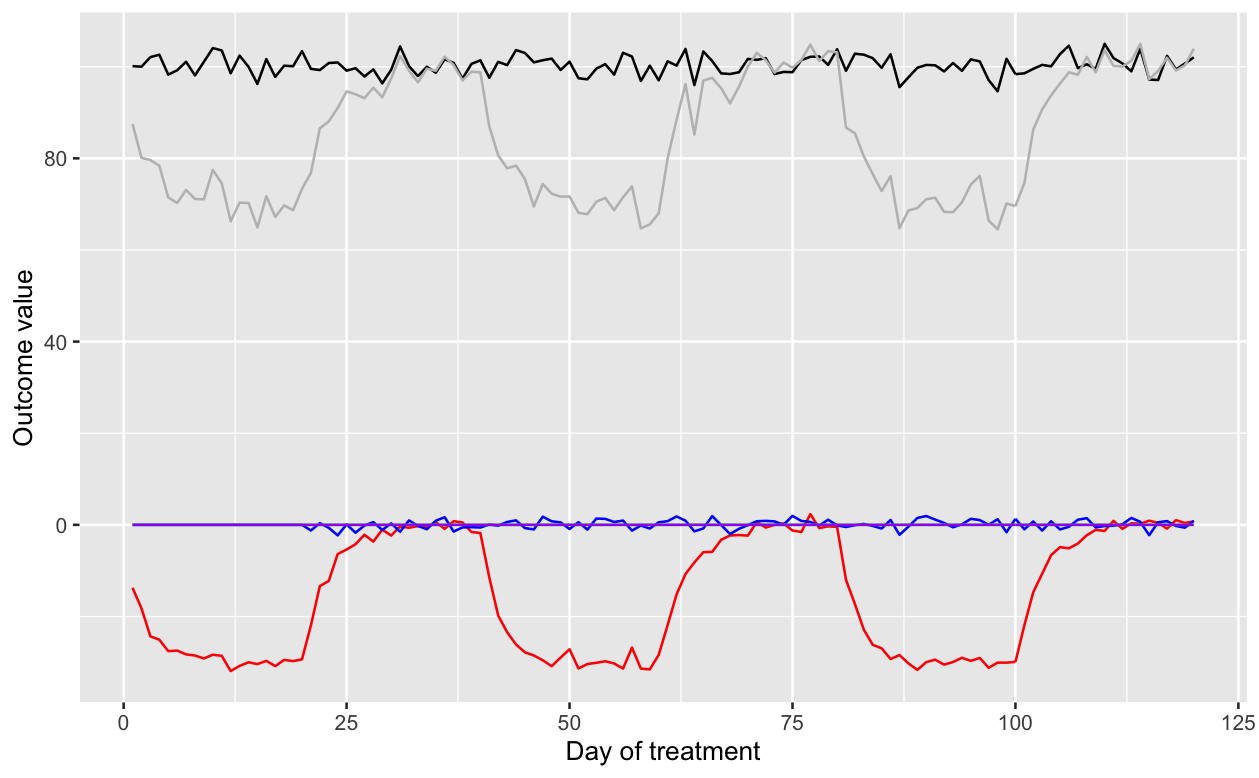
\includegraphics[width=0.8\linewidth]{./img/simulation-output} 

}

\caption{An example simulation output. Baseline value was initialized at 100 with $\sigma_b^2 = 5$. Treatment A (red) has a true effect of -30 with a carryover constant of 2, run-in constant of 2 and $\sigma^2_A = 1$. Treatment B (blue) is a placebo with no treatment effect 0, no carryover or run-in and $\sigma^2_B = 1$. Other treatments (C) were not specified and do not contribute to the observed effect.}\label{fig:unnamed-chunk-2}
\end{figure}

\subsection{Simulation Scope}\label{simulation-scope}

For the purposes of limiting the scope of term paper, we have chosen not
to model particular important aspects of an N-of-1 trial. We have chosen
not to model potential interactions between treatments and long-term
time trends in the clinical outcome that are commonly seen in trials.
Some trials incorporate wash-out periods to account for run-in, but this
was not included in our software. Since we are focusing on design and
treatment parameters, we have not modeled patient-specific
autocorrelation in the simulation process.

\subsection{Statistical Analyses}\label{statistical-analyses}

For our analyses, we have chosen to perform regression analyses as
recommended by Kravitz et. al in the AHRQ Handbook {[}1{]}. The clinical
outcome will be modeled as a linear function of \(T-1\) indicator
variables for each treatment using a placebo as the reference and
\(B-1\) indicator variables for each block using the first block as the
reference. The model can be written as:

\[
Y_{kb} = \beta_0 + \beta'_1 \mathbf{T} +\beta_2'\mathbf{B} + \epsilon_{kb}
\]

where \(\mathbf{T}\) is the matrix of treatment indicator variables
indexed by \(k\) and \(\mathbf{B}\) is the matrix of block indicators
indexed by \(b\). After some exploratory analytical testing, we found
this model to provide accurate estimates while remainining estimable. We
attempted to use linear mixed-effects models, but we found that we were
not generating enough data for the models to converge.

A significant result in a simulation is defined as when the regression
coefficient associated with the active treatment to be significant
(\(p < 0.05\)). Overall power of a given set of simulations was defined
as the proportion of which obtain a significant result for the active
treatment. Finally, we define the probability of correct selection (PCS)
as the proportion of simulation trials where the resulting coefficient
estimate for treatment satisfies a pre-specified condition, such as
maximization of effect or choosing the treatment that avoids unnecessary
under- or over-treatment.

For our study, we investigate how different sets of design and treatment
parameters have the potential to affect the overall power, effect
estimation and PCS. We use this criteria as a balance between
researchers who may want to maximize power and accurate estimation
against patient interests, who will want to find the correct treatment
as soon as possible while minimizing harm and cost.

\subsection{Performance Metrics}\label{performance-metrics}

Our case study highlights just one use case for N-of-1 trials. For our
paper, we chose to use three performance metrics to explore how
different parameters affect the needs of a trial: average power, average
deviation and probability of correct selection (PCS). All performance
metrics were calculated from the results of 100 simulations, given a set
of treatment parameters. For power, a linear model was created after
each simulation, and the significance of the treatment was checked.
Average power was calculated as the proportion of the 100 simulations
that found the treatment to be significant. For average deviation, the
deviation away from the (known) true effect was calculated from the
model estimate. Average deviation was calculated as the mean deviation
of the 100 simulations. PCS was calculated under a particular selection
criteria. For our paper, we explored two different criteria for correct
selection: 1) correct when choosing the treatment with maximal effect
and 2) correct when choosing the treatment that most accurately
estimates an effect within a given window of acceptable effect. PCS was
calculated as the proportion of simulations that correctly select the
known optimal treatment.

\section{Results}\label{results}

\subsection{Case Study: Active Treatment vs
Placebo}\label{case-study-active-treatment-vs-placebo}

To demonstrate the nuances of design consideration, we present a case
study using our simulations. We assume two treatments with a continuous
outcome measurement: \(A\) has a treatment effect of -3 with 2 run-in
and 2 carryover days. \(B\) is the placebo with 0 treatment effect and
has 1 run-in and 1 carryover day (Figure 2). Our choice of tuning design
parameters resulted in the following simulation scenarios:

\begin{enumerate}
\def\labelenumi{\arabic{enumi}.}
\tightlist
\item
  Treatment selection: \(ABAB\), \(ABBA\), \(BABA\), \(BAAB\) holding
  sampling frequency to 1, period length to 5 days, and the number of
  blocks to 2
\item
  Sampling frequency: 1 to 30 times in a period holding treatment order
  to \(ABAB\), period length to 5 days, and the number of blocks to 2
\item
  Period length: 2-120 days holding treatment order to \(ABAB\),
  sampling frequency to 1 per period, and the number of blocks to 2
\item
  Number of blocks: 1-6 blocks holding treatment order to \(ABAB\),
  sampling frequency to 1 per period, and period length to 5 days
\end{enumerate}

Figure 2 was derived from simulating each scenario and parameter 50
times. Effect estimates were calculated from regression adjusting for
block number as described previously. The median value of effect
estimates were calculated from statistically significant regression
estimates and used for comparison.

From Figure 2, the treatment order \(ABBA\) has the closest estimate of
treatment effect with a median of -2.45 and variance of 0.18. The
differences in treatment effect are likely a result of the carryover and
run-in effects. Given that our simulation assumed 5 day periods and
sampled once a period, carryover and run-in effects become prominent.

Increasing sampling frequency results in higher accuracy of treatment
effect with decreasing variance. However, from Figure 2, the increased
sampling frequency has diminishing results and the best estimates
started to plateau. Around 5 samples in a 5 day period results in a
median treatment effect of -2.83 with a 0.04 variance while 10 samples
in a 5 day period results in a median treatment effect of -2.91 with a
0.02 variance. Sampling can be invasive to a patient but critical to
power of the study. This simulation demonstrates that it is possible to
identify a lower sampling frequency without compromising the best
estimate of treatment effect.

Like sampling frequency, increasing period length increases accuracy of
treatment effect estimation over time along with decreasing variance.
From Figure 2, treatment effect plateaus between period lengths of 15 to
30 days, where median treatment effects are -2.70 and -2.90
respectively. Again, large period lengths can be exhaustive to a
patient, especially if there are negative side effects involved.
Minimizing period length while still maintaining power and effect
estimate are important steps to consider. It should also be noted from
Figure 2 that the results when period length is 2 days are not
significant. This is probably a result of low power in addition to
carryover and run-in effects. Effects from treatment A and B likely run
into each other within the span of two days.

We varied block length and in Figure 2 we observe no significant
difference in effect estimate with increasing blocks. However, variance
does decrease with increased blocks. We surmise that the reason we do
not observe any differences is that our simulation does not model
time-trends. We do observe variance decreased because sample size
increases with blocks thereby increasing certainty in the estimates.

\begin{figure}

{\centering 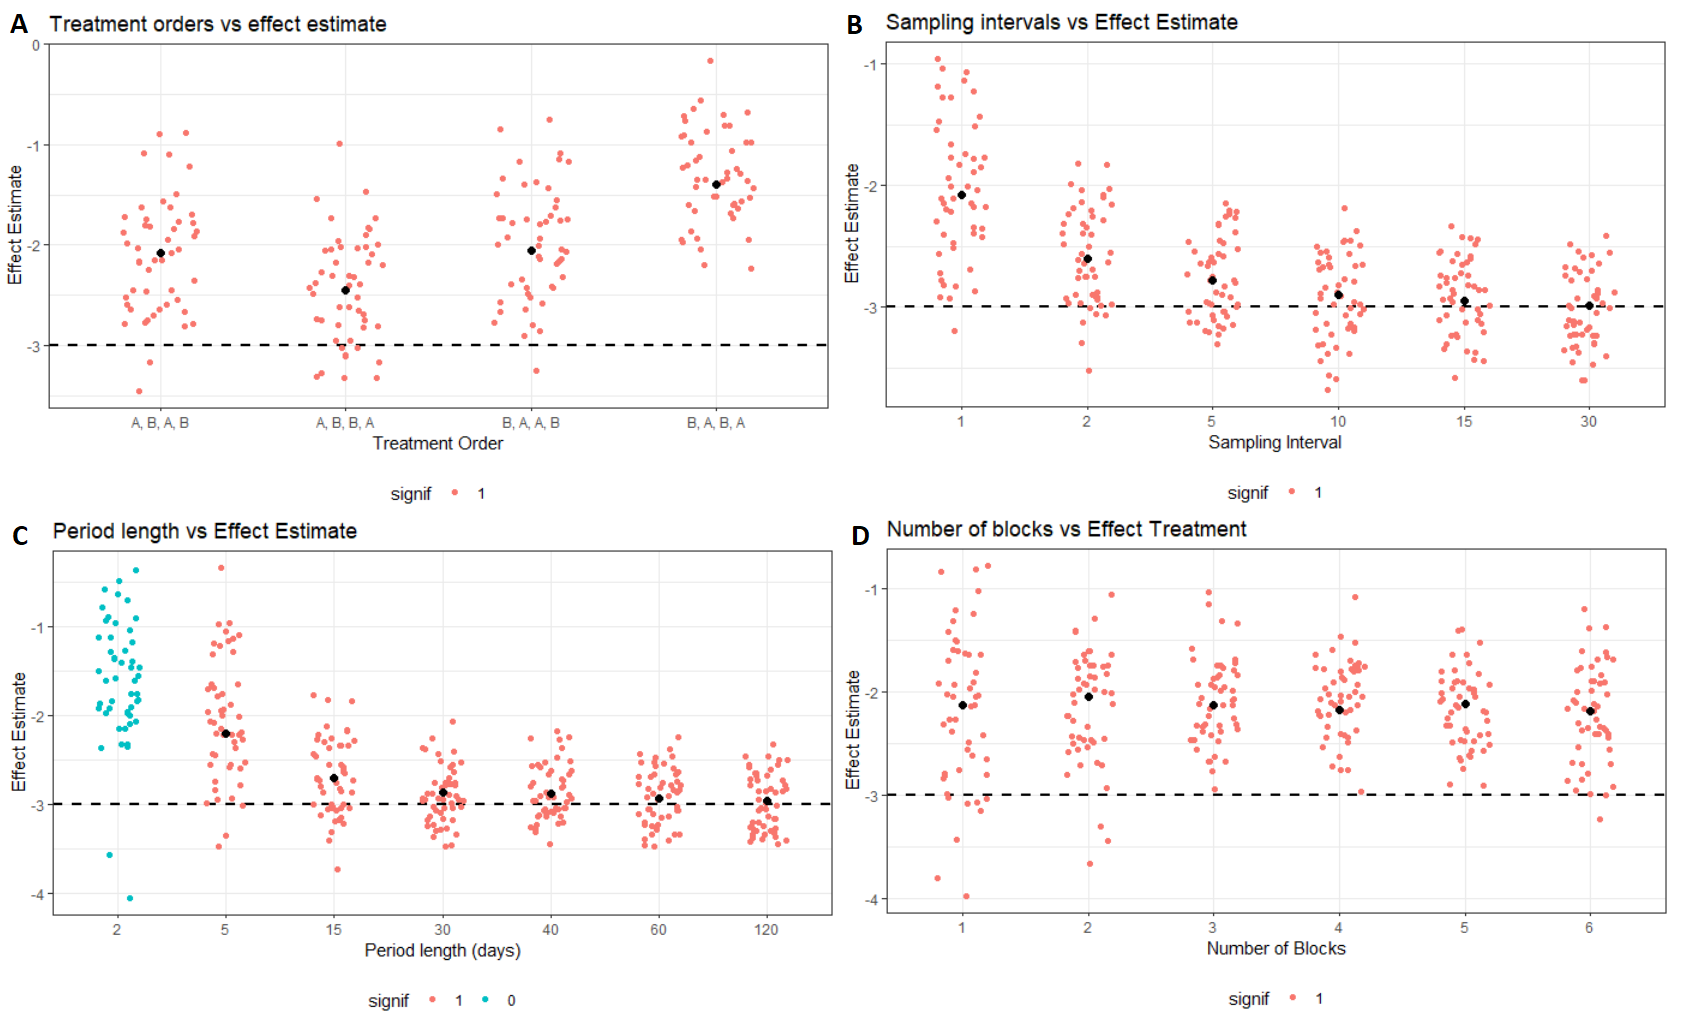
\includegraphics[width=0.8\linewidth]{./img/combined_case_study} 

}

\caption{Simulation results on effect estimate after tuning for design parameters, including (A) treatment orders, (B) sampling frequency, (C) period length, (D) number of blocks. Each tuning parameter was run with 50 simulations. Drug A has a true effect of -3 while Drug B is a placebo with 0 effect. Black points are median effect sizes among statistically significant results.}\label{fig:unnamed-chunk-3}
\end{figure}

\subsection{Sample Size \& Power}\label{sample-size-power}

\begin{figure}

{\centering 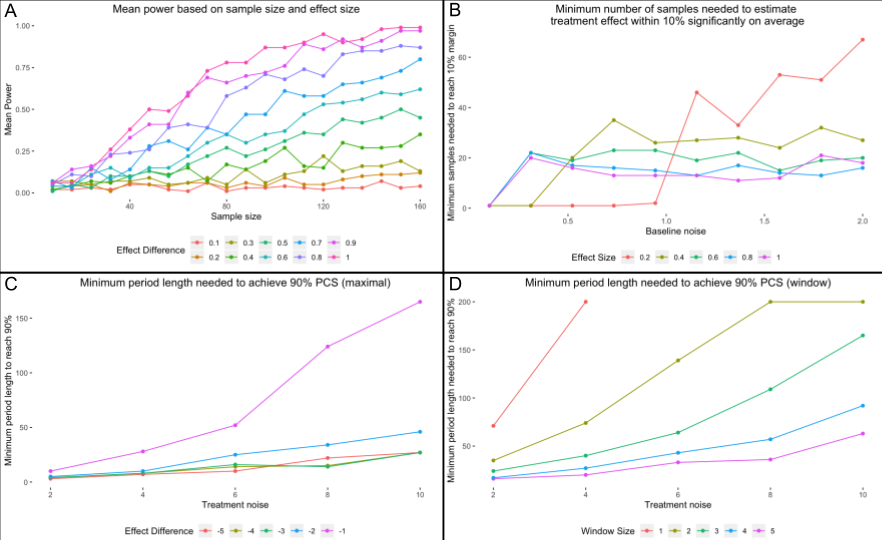
\includegraphics[width=0.9\linewidth]{./img/term-paper-fig-3} 

}

\caption{Simulations showing how varying treatment parameters affects power, treatment effect estimation and PCS.}\label{fig:unnamed-chunk-4}
\end{figure}

Figure 3a is the result of a series of simulations designed to
investigate the effect of changes to treatment effect sizes on average
power and effect estimation. We kept the number of blocks constant at 2
and the treatment order at \(ABBA\) (\(A\) being the active treatment,
\(B\) being placebo). The initial baseline value was 0, and baseline
noise was set to 1. For these simulations, the effect of the active
treatment was a linear function of the baseline noise. The active
treatment was given carryover and run-in constants of 2 and a negligible
noise. Keeping sampling frequency at 1/period and looking at different
period lengths from 1 to 20 days, we looked at the average power for a
set of 100 simulations. We have a supplemental table at the end laying
out the simulation parameters used for each figure.

The result is a trend line that shows the relationship between the final
sample size the resulting power from that sample size, stratified by
different effect sizes. We observed that for extremely small effect
sizes (\textless{} 0.5) that trials must be extremely long to detect a
meaningful effect. For the largest effect size we simulated, we observed
that a sample size of about 80 measurements was needed to reach 80\% and
about 110 to reach 90\% power. This equates to a period length of about
10.

\subsection{Minimum Sample Size \& Average
Deviation}\label{minimum-sample-size-average-deviation}

Figure 3b shows the result of simulations designed to look at the
minimum sample size needed to accurately estimate the true treatment
effect on average. ``Accurate estimation'' was defined as the mean
deviation between the estimated treatment effect and the true effect
across 100 simulations. The design and treatment parameters were kept
the same as in the sample size and power simulations. Keeping sampling
frequency at 1, period length was increased until the average deviation
was within 10\% of the true effect. This process was repeated for
different effect sizes. We found that a sample size of about 50 was
enough to accurately estimate the treatment effect, even as baseline
noise increased. However, for extremely small effects, the necessary
sample size for accurate estimation jumped to about 100.

\subsection{Selection for maximal
effect}\label{selection-for-maximal-effect}

Figure 3c looks at simulations done to investigate how well an N-of-1
trial is able to correctly choose between two competing treatments. Out
of 100 simulations for a given a combination of treatment noise and
difference in treatment effects, we calculated the PCS. The design
parameters were kept the same as in 2a and 2b, except for treatment
order. A placebo was used as a third treatment, and the order was the
two active treatments followed by the placebo. The optimal active
treatment had a reducing effect of 5. Both active treatments had run-in
and carryover constants of 2. We observe that for small absolute
differences in the competing treatment effects that especially large
sample sizes are needed to detect the effect. For example, an effect
size of 1 corresponds to a period length of 33 is needed to correctly
choose the best treatment 90\% of the time. As the effect difference
increases, the necessary sample size to achieve a PCS of 90\% seems to
level off at about a period length of 20.

\subsection{Selection in an optimal treatment
window}\label{selection-in-an-optimal-treatment-window}

Figure 3d examines a different definition of probability of correct
selection. For these simulations, there were 3 competing active
treatments, accompanied by a placebo. One treatment was considered
optimal, while the other two had treatment effects that represented both
under- and over-treatment. We investigated the minimum sample size
required to correctly identify the optimal treatment 90\% of the time
over 100 simulations. The optimal treatment effect was known, and a
treatment was selected based on the smallest deviation from this known
effect. Sampling frequency was kept at 1 per period, and the treatment
order was set at: optimal, under-treatment, over-treatment, then
placebo. All active treatments had the same noise, carryover and run-in.
The initial baseline parameters were the same for the previous treatment
selection simulation.

We observed that for small windows of efficacy (effect differences ± 1,
2) the minimum sample size necessary to pick out the optimal treatment
grows roughly exponentially as the treatment noise increases. We chose
to limit the number of candidate sample sizes to 200, which we see is
reached by the small window sizes. For more generous windows, the
exponential increase is slowed. For an effect size of 1
(\(\sigma_t^2 = 5\)), we see that a minimum sample size of about 50
observations is needed to correctly select the best treatment 90\% of
the time. From the treatment order and number of blocks, this translates
to a period length of about 7 days per treatment.

\section{Discussion}\label{discussion}

\subsection{Study Intent}\label{study-intent}

The purpose of our study was to use simulation to investigate how
different treatment parameters have the potential to affect important
statistical and clinical endpoints, which have the potential to be at
odds with each other. A statistician may desire the extension of a study
for the purposes of power and accurate estimation, but this may come at
the cost of higher patient attrition or extended exposure to treatment
side-effects. Simulation is a powerful tool for allowing researchers to
better plan out their designs in hopes of striking a balance between
these two realities, but as we have discovered over the course of this
project, this benefit is only as good as the realism of the simulation
itself. We hoped to extend the work of Percha et. al to treatment
selection and non-ideal cases where carryover and run-in effects are
present.

\subsection{Recommendations}\label{recommendations}

\subsubsection{Case Study}\label{case-study}

Within our simulations, we confirm that treatment order, sampling
frequency, and period length to be important design considerations. Had
our simulation included time-trends, we expect block length to be
critical as well. We noticed the simulations were strongly influenced by
wash-in and carryover effects, so we would recommend considering washout
periods between treatments or consider sampling after treatment effects
are stabilized to decrease these effects. Period length and sampling
frequency should be balanced in a way that allows for accurate treatment
selection without making the trial unnecessarily long. Our case study
demonstrates the importance of simulations in their ability to decompose
complex design and environmental factors to better understand how
analysis can be maximized without compromising the patient's healthcare.

\subsubsection{Power}\label{power}

The length of the N-of-1 trial is the sole determinant of the sample
size, and researchers are able to change their sample size by tuning the
design parameters. From our simulation findings, we observe that N-of-1
trials run a high risk of being highly underpowered, especially in cases
where the active treatment does not do much better than the placebo or
when the clinical outcome of interest is highly variable. It is no
surprise that researchers must try to make as many observations as
possible to achieve acceptable power, but it is helpful to keep a sort
of minimum necessary sample size to have some confidence in truly
detecting effective treatments. For larger effects, we found that sample
sizes of about 80 observations were enough to start approaching 80\%
power. With this in mind, researchers designing N-of-1 trials should be
prepared to conduct studies spanning 3-4 months, assuming one
observation per day. Shorter trials may still be effective at accurately
estimating the treatment effect, but these effects may not be truly
significant.

\subsubsection{Probability of Correct
Selection}\label{probability-of-correct-selection}

Our simulations find that the definition of ``correct' treatment
selection has critical implications on the necessary sample size needed
to identify the correct treatment for a patient. In simple cases where
we are only seeking the treatment with maximal effect, period length of
about 50 seem to suffice in correctly identifying the maximal treatment
effect, even in cases where the treatment noise is large.

This is not the case when we must avoid both under-treatment and
over-treatment. This problem may arise in cases where an adequate
treatment is known, but the correct dose to use is not. Compared to the
corresponding line in Figure 3c, having to account for a window
necessitates a greater period length to avoid under- or over-treatment.
This difference in sample size is even greater when the exact window for
optimal treatment is small. For example, even for effect sizes of 2
(\(\sigma_t^2 = 2.5\)), the necessary period length to identify a
maximal treatment effect is about 25, compared to about 150 needed to
identify it in a window. This finding highlights the fact that including
more treatments necessitates greater sample size to accurately estimate
each of their effects. Researchers should carefully define their goal in
correctly selecting a treatment for a subject since it can greatly alter
the resulting design that is needed to achieve it.

\subsubsection{Effect Estimation}\label{effect-estimation}

In terms of the three performance metrics we chose to examine, accurate
treatment effect estimation may not hold as much importance in an N-of-1
trial. Despite this, we still feel that accurate estimation of treatment
effects has critical implications in proper treatment selection. As
mentioned before, our simulations found that N-of-1 trials tend to
estimate treatment effects accurately faster than they do achieve
statistical power. This finding might be useful in cases where it is
unknown how a subject will react to treatment. To start estimating the
true treatment effect, sample sizes of about 20 observations are needed.
This information might be useful to researchers to motivate a
reevaluation of the trial design after the effects are estimated, much
like an internal pilot.

These findings highlight a looming logistical problem with N-of-1
trials. More reasonable trial lengths from a patient perspective are
more likely than not to be underpowered and have biased estimates of the
treatment effect. Researchers should combine simulation use and patient
consultation to work towards a compromise that fits both their and
patient needs. Our simulations also demonstrate that acceptable
performance metrics are met when the treatment effects are similar in
magnitude to baseline or treatment noise; in cases where these effects
are small, researchers may want to discuss the pros and cons of extended
treatment regimens for effects that may not be clinically relevant for
the patient.

\subsection{Limitations}\label{limitations}

For our project, we made several simulation design choices to limit the
scope of our project. We chose to emulate much of our simulation after
the Percha study, but we made some changes based on time constraints. We
model a baseline clinical outcome as a Markov process to represent a
subject outcome of interest in the absence of any treatment. We ignore
any longer time trends such as drift or cyclicality, which are apparent
in many important biological phenomena. Furthermore, in our simulations,
we have only chosen a small subset of parameters in a vast parameter
space, so our findings may differ greatly in other contexts. For
example, long carryover and run-in have immediate consequences on proper
treatment selection, which may motivate a researcher to incorporate a
washout period.

\subsection{Group Reflection}\label{group-reflection}

This project gave us an increased appreciation for the role of
simulation in guiding research. We've been exposed to the use of
simulation in evaluating statistical techniques in Prof.~Wei's Topics in
Computing Class, but this is the first time we've seen it used in a
clinical trial context. Although we were unable to incorporate more
Bayesian or adaptive techniques into our analytic plan, we feel that the
framework we laid out can easily be extended to accommodate this type of
analysis. Although we're proud of the work done here, there's a lot of
room for refinement. In the end, both Adina and I appreciate the N-of-1
studies as an alternative to other study-designs we've been exposed to.
They are dizzingly complex and each individual study will have different
aspects to take into consideration, but at least this is where
simulation can help to tease through these difficult decisions.

\pagebreak

\section{References}\label{references}

\begin{enumerate}
\def\labelenumi{\arabic{enumi}.}
\tightlist
\item
  Kravitz RL, Duan N, eds, and the DEcIDE Methods Center N-of-1 Guidance
  Panel (Duan N, Eslick I, Gabler NB, Kaplan HC, Kravitz RL, Larson EB,
  Pace WD, Schmid CH, Sim I, Vohra S). Design and Implementation of
  N-of-1 Trials: A User's Guide. AHRQ Publication No. 13(14)-EHC122-EF.
  Rockville, MD: Agency for Healthcare Research and Quality; January
  2014.
\item
  Percha B, Baskerville EB, Johnson M, Dudley JT, Zimmerman N. Designing
  Robust N-of-1 Studies for Precision Medicine: Simulation Study and
  Design Recommendations. J Med Internet Res 2019;21(4):e12641
\end{enumerate}

\pagebreak

\begin{table}[t]

\caption{\label{tab:supplement-tbl}(Supplement)Parameters used in different simulations for Figure 3}
\centering
\fontsize{9}{11}\selectfont
\begin{tabu} to \linewidth {>{\raggedright}X>{\raggedright}X>{\raggedright}X>{\raggedright}X>{\raggedright}X>{\raggedright}X}
\toprule
Parameter & Notation & 2a & 2b & 2c & 2d\\
\midrule
\rowcolor{gray!6}  Sampling Frequency & $F$ & 1 & 1 & 1 & 1\\
 
Period Length & $P$ & Varies & Varies & Varies & Varies\\
 
\rowcolor{gray!6}  Number of Treatments & $T$ & 2 & 2 & 3 & 4\\
 
Treatment Order & $O$ & A, B, B, A & A, B, B, A & A, B, C & A, B, C, D\\
 
\rowcolor{gray!6}  Number of Blocks & $B$ & 2 & 2 & 2 & 2\\
 
Treatment Effect & $E_k$ & Varies & Varies & -5, Varies & -5, Others Varies\\
 
\rowcolor{gray!6}  Carryover & $\tau_k$ & 2 & 2 & 2 & 2\\
 
Run-in & $\gamma_k$ & 2 & 2 & 2 & 2\\
 
\rowcolor{gray!6}  Treatment Noise & $\sigma^2_k$ & 0.01 & 0.01 & Varies & Varies\\
 
Baseline Start & $\mu_b$ & 0 & 0 & 100 & 100\\
 
\rowcolor{gray!6}  Baseline Noise & $\sigma^2_b$ & 1 & Varies & 1 & 1\\
 
Number simulations & $N$ & 100 & 100 & 100 & 100\\
\bottomrule
\end{tabu}
\end{table}


\end{document}
